{
	\setbeamertemplate{background}{\tikz[overlay,remember picture]\node[opacity=0.4]at (current page.center){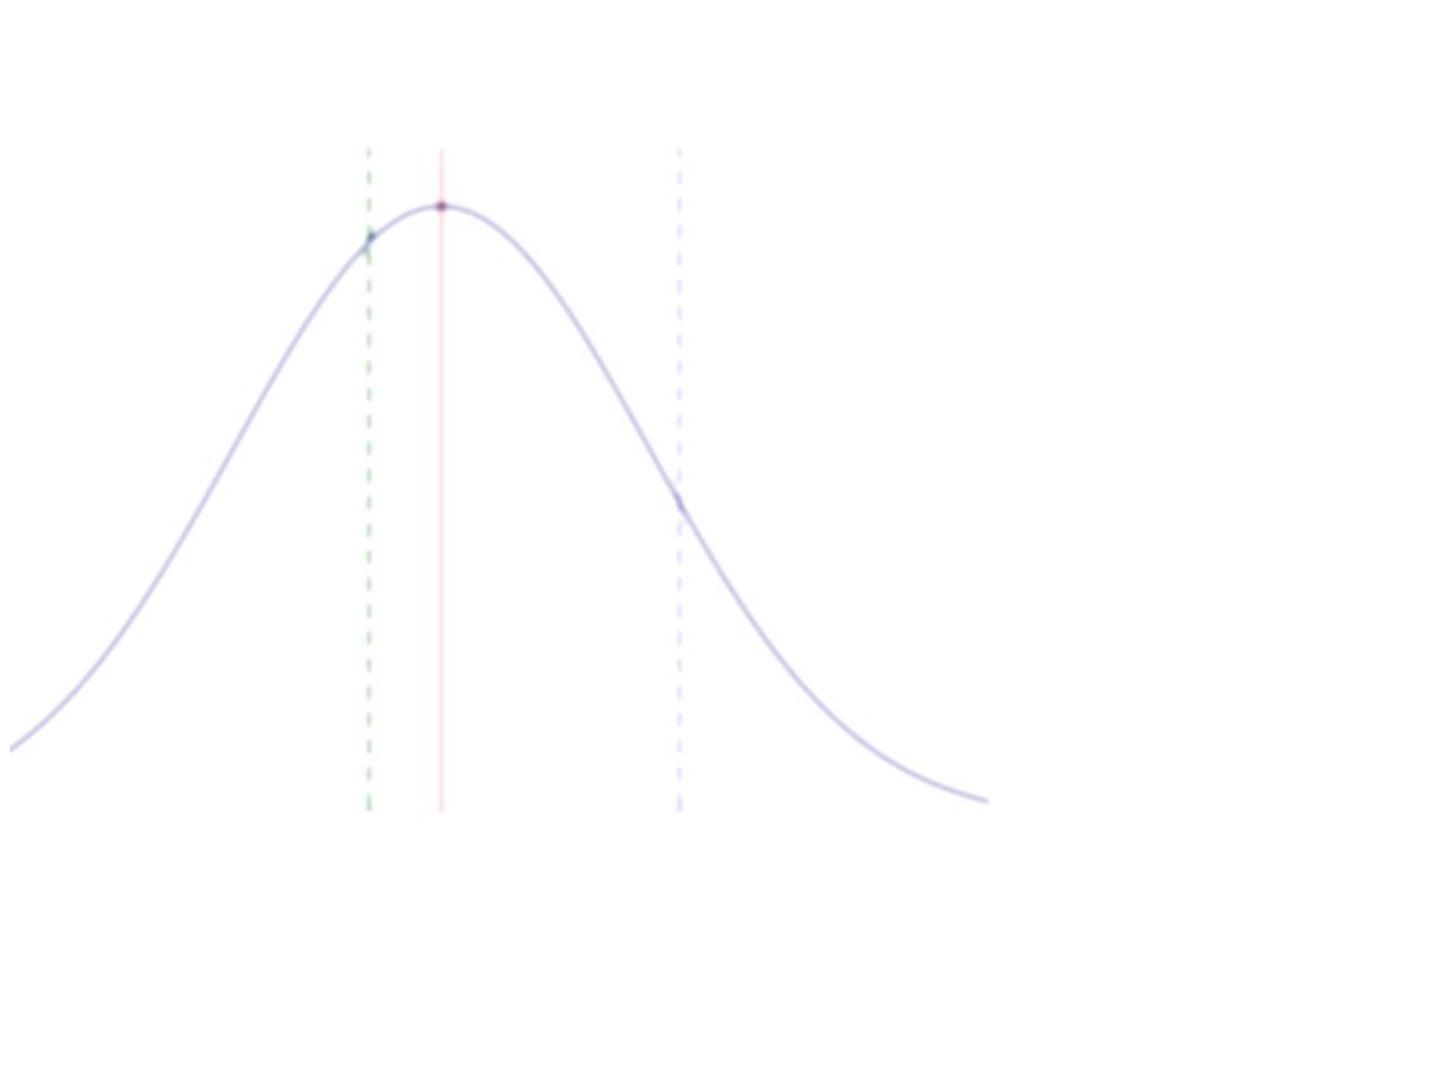
\includegraphics[width=13cm]{../../material/Econometrics.png}};}
	
	\begin{frame}[noframenumbering,plain] % Omits frame-numbering --> include \addtocounter{framenumber}{-1} at the following frame
	\begin{picture}(320,250)
	% Github Logo
	\put(-2,8){\href{https://github.com/HumanCapitalEconomics/talks/tree/master/distribution}{
\includegraphics[height=0.8cm]{../../material/GithubMarkCS.png}}}
	% Github Text
	\put(-12,38){\begin{minipage}[t]{0.4\linewidth}
		{\small {\color{darkgray!85!blue}{\tiny{Material available on}}}}
		\end{minipage}}
	\put(5.5,6){\begin{minipage}[t]{0.4\linewidth}
		{\small {\color{darkgray!85!blue}{\tiny{Visit us!}}}}
		\end{minipage}}
	% Uni Bonn Logo 
	\put(230,0){
\includegraphics[height=1cm]{../../material/UniBonnLogo.png}}
	% Cover Text and Author
	\put(180,230){\begin{minipage}[t]{0.4\linewidth}
		{{\color{darkgray!85!blue}{ \Huge {\slshape E}}}{{\color{darkgray}\large \slshape conometrics}} \\ \vspace{-5.5pt} \\
			{\color{darkgray}\slshape of} { {\color{darkgray!85!blue}\Huge {\slshape H}}}{{\color{darkgray}\large \slshape uman}} \\ \vspace{-5.5pt} \\
			{{\color{darkgray!85!blue} \Huge {\slshape C}}}{{\color{darkgray}\large \slshape apital}}
			\hspace{2pt} {\color{orange!45!yellow}\rule[-0.5mm]{60mm}{0.25mm}}
			$~~~~~$ {\color{darkgray!85!blue}Philipp Eisenhauer}}
		\end{minipage}}
\end{picture}
\end{frame}
}